% ---------------------------------------------------------------- 6
\begin{frame}{Objectifs pédagogiques du chapitre}
\begin{columns}[t]
\begin{column}{0.48\textwidth}
\begin{kbox}[Savoirs]
\begin{itemize}
  \item Distinguer les deux interprétations de la probabilité
  \item Énoncer et démontrer le théorème de Bayes
  \item Définir prior, vraisemblance, posterior, prédictive
  \item Lire un intervalle de crédibilité
\end{itemize}
\end{kbox}
\end{column}
\begin{column}{0.48\textwidth}
\begin{abox}[Savoir-faire évalués]
\begin{itemize}
  \item Calculer un posterior conjugué à la main
  \item \textbf{Écrire et exécuter} un modèle PyMC
  \item Produire un graphique de posterior exploitable
  \item Critiquer un prior (trop informatif ? justifié ?)
\end{itemize}
\end{abox}
\end{column}
\end{columns}
\vspace{2mm}
\begin{tcolorbox}[colback=byLight,colframe=byGrey!50,arc=2mm,width=.95\textwidth]
\centering\small
\textbf{Évaluation} — contrôle continu 30 \% (TP noté + quiz) \;|\; examen final écrit 70 \%.
\end{tcolorbox}
\end{frame}

% ---------------------------------------------------------------- 7
\begin{frame}{Plan du chapitre 1 (8 h)}
\begin{enumerate}
  \item[1.1] \textbf{Contexte et motivation} \hfill \textit{slides 2--8}
  \item[1.2] \textbf{Probabilité : deux interprétations} \hfill \textit{slides 9--20}
  \item[1.3] \textbf{Le théorème de Bayes et sa mécanique} \hfill \textit{slides 21--34}
  \item[1.4] \textbf{Bayésien contre fréquentiste} \hfill \textit{slides 35--44}
  \item[1.5] \textbf{L'écosystème logiciel et le premier modèle} \hfill \textit{slides 45--50}
\end{enumerate}
\vspace{3mm}
\begin{tabular}{@{}llll@{}}
\toprule
\textbf{Volume} & \textbf{Cours magistral} & \textbf{TD} & \textbf{TP machine} \\
\midrule
8 h & 5 h & 1 h 30 & 1 h 30 \\
\bottomrule
\end{tabular}
\vspace{2mm}
\begin{tcolorbox}[colback=byPurple!6,colframe=byPurple,arc=2mm,width=.95\textwidth]
\small\centering
\textbf{Prérequis mobilisés} : probabilités conditionnelles, loi binomiale et normale,
$\int_0^1 x^{a-1}(1-x)^{b-1}\mathrm{d}x$, Python.
\end{tcolorbox}
\end{frame}

% ---------------------------------------------------------------- 8
\begin{frame}{Activité brise-glace — tour de table (5 min)}
\begin{abox}[Consigne]
Chacun cite \textbf{une décision incertaine} de son domaine, en une phrase, puis indique
\textbf{ce qu'il savait déjà} avant de voir les données.
\end{abox}
\vspace{1mm}
\begin{columns}[t]
\begin{column}{0.31\textwidth}
\begin{ebox}[Santé]
« Ce traitement marche-t-il sur 12 patients ? »
\vspace{1mm}
\footnotesize Ce qu'on sait : les essais antérieurs, la physiologie.
\end{ebox}
\end{column}
\begin{column}{0.31\textwidth}
\begin{ebox}[Industrie / Web]
« Ce bouton augmente-t-il le taux de clic ? »
\vspace{1mm}
\footnotesize Ce qu'on sait : les A/B tests passés, la taille d'effet plausible.
\end{ebox}
\end{column}
\begin{column}{0.31\textwidth}
\begin{ebox}[Recommandation]
« Ce film va-t-il plaire ? »
\vspace{1mm}
\footnotesize Ce qu'on sait : les goûts déclarés, les notes globales.
\end{ebox}
\end{column}
\end{columns}
\vspace{2mm}
\begin{kbox}[Ce que l'on va apprendre à faire]
Transformer la colonne « ce qu'on sait » en une \textbf{loi a priori}, puis la
confronter aux données sans jeter ni l'un ni l'autre.
\end{kbox}
\end{frame}

% ---------------------------------------------------------------- 9
\begin{frame}{Deux visions de la probabilité}
\begin{columns}[t]
\begin{column}{0.48\textwidth}
\begin{tcolorbox}[enhanced,colback=byRed!7,colframe=byRed,arc=2mm,
   title={\bfseries\color{white} Fréquentiste},colbacktitle=byRed,
   attach boxed title to top left={xshift=3mm,yshift=-2mm},
   boxed title style={arc=1mm,boxrule=0pt}]
\begin{itemize}
  \item Probabilité = \textbf{fréquence de long terme} d'un événement répétable
  \item Le paramètre $\theta$ est \textbf{fixe et inconnu}
  \item On raisonne sur la variabilité des \textbf{échantillons}
  \item Outils : $p$-value, intervalle de confiance, puissance
  \item Phrase type : « si je répétais 1000 fois l'expérience, dans 95 \% des cas… »
\end{itemize}
\end{tcolorbox}
\end{column}
\begin{column}{0.48\textwidth}
\begin{tcolorbox}[enhanced,colback=byBlue!7,colframe=byBlue,arc=2mm,
   title={\bfseries\color{white} Bayésien},colbacktitle=byBlue,
   attach boxed title to top left={xshift=3mm,yshift=-2mm},
   boxed title style={arc=1mm,boxrule=0pt}]
\begin{itemize}
  \item Probabilité = \textbf{degré de croyance} cohérent (\textit{plausibilité})
  \item Le paramètre $\theta$ est \textbf{aléatoire}, décrit par une loi
  \item On raisonne sur la variabilité du \textbf{paramètre}
  \item Outils : distribution a posteriori, intervalle de crédibilité
  \item Phrase type : « il y a 95 \% de chance que $\theta$ soit dans… »
\end{itemize}
\end{tcolorbox}
\end{column}
\end{columns}
\vspace{1.5mm}
\centering\small
Les deux écoles utilisent \textbf{les mêmes probabilités conditionnelles} :
elles diffèrent sur \textit{ce qui est aléatoire}.
\end{frame}

% ---------------------------------------------------------------- 10
% [split]
\begin{frame}{Ce que dit une fréquence, et ce qu'elle ne dit pas}
\begin{center}
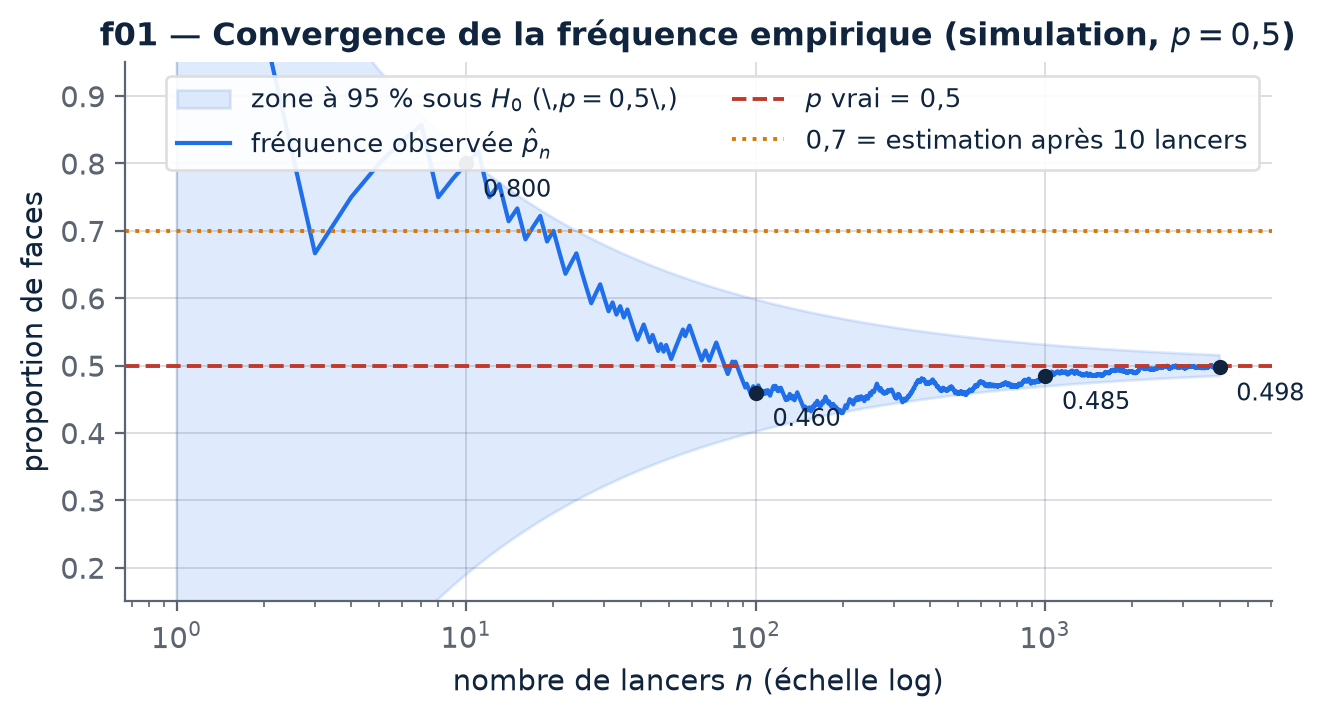
\includegraphics[width=.86\textwidth]{f01_convergence_frequence.png}
\end{center}
\end{frame}

% [split]
\begin{frame}{Ce que dit une fréquence, et ce qu'elle ne dit pas}

\vspace{-1mm}
\begin{columns}[t]
\begin{column}{0.54\textwidth}
\begin{ebox}[Lecture des données simulées]
Après 10 lancers on observe $\hat p = $ \textbf{0,80}. Après 4000 lancers : \textbf{0,498}.
Le fréquentiste conclut : \emph{« la fréquence converge vers $p$ ; la valeur
0,80 n'est qu'une fluctuation »} — mais il ne peut pas parler de $P(0{,}45 < p < 0{,}55)$\dots
\end{ebox}
\end{column}
\begin{column}{0.42\textwidth}
\begin{wbox}[Le piège fréquentiste]
\begin{itemize}
  \item $p$ n'est pas une variable : aucune probabilité ne lui est attachée.
  \item L'IC à 95 \% est \textbf{un long terme théorique}, pas la confiance dans
        \emph{cet} intervalle calculé.
  \item Aucun moyen d'injecter le fait que la pièce semble équilibrée \textit{a priori}.
\end{itemize}
\end{wbox}
\end{column}
\end{columns}
\end{frame}

% ---------------------------------------------------------------- 11
\begin{frame}{La probabilité comme état de connaissance}
\begin{kbox}[Postulat bayésien]
Une probabilité est une \textbf{appréciation de plausibilité par un agent} cohérent.
Deux agents avec des informations différentes \emph{doivent} avoir des probabilités
différentes — et c'est une force, à condition de dire lesquelles.
\end{kbox}
\vspace{2mm}
\begin{columns}[t]
\begin{column}{0.48\textwidth}
\begin{ebox}[Exemple 1 — question piégée]
« Quelle est la probabilité que la Chine soit le premier pays à poser un humain sur Mars ? »
\vspace{1mm}
\footnotesize Il n'y a pas de « fréquence de long terme » : l'événement est unique.
Pourtant on sait raisonner, comparer, mettre à jour.
\end{ebox}
\end{column}
\begin{column}{0.48\textwidth}
\begin{ebox}[Exemple 2 — l'ordre]
« Ce patient a survécu 3 mois au traitement. »
\vspace{1mm}
\footnotesize Le bayésien peut arrêter l'essai quand les données le justifient
(interprétation \textit{conditionnelle} aux données observées),
sans gonfler artificiellement le risque de première espèce.
\end{ebox}
\end{column}
\end{columns}
\vspace{1.5mm}
\begin{tcolorbox}[colback=byCyan!8,colframe=byCyan,arc=2mm,width=.95\textwidth]
\small\centering
\textbf{Conséquence pratique :} la conclusion bayésienne s'énonce
\textbf{conditionnellement aux données réellement observées} — pas sur des
répétitions imaginaires de l'expérience.
\end{tcolorbox}
\end{frame}

% ---------------------------------------------------------------- 12
\begin{frame}{Mise à jour séquentielle : le cœur du raisonnement}
\begin{ebox}[Principe]
Le posterior d'aujourd'hui devient le prior de demain :
$p(\theta \given y_1, y_2) \neq$ refaire tout le calcul, mais
$p(\theta \given y_1, y_2) \propto p(\theta) \, p(y_1 \given \theta) \, p(y_2 \given \theta)$.
L'ordre d'arrivée des données \textbf{ne change pas} le résultat.
\end{ebox}
\vspace{1mm}
\begin{center}
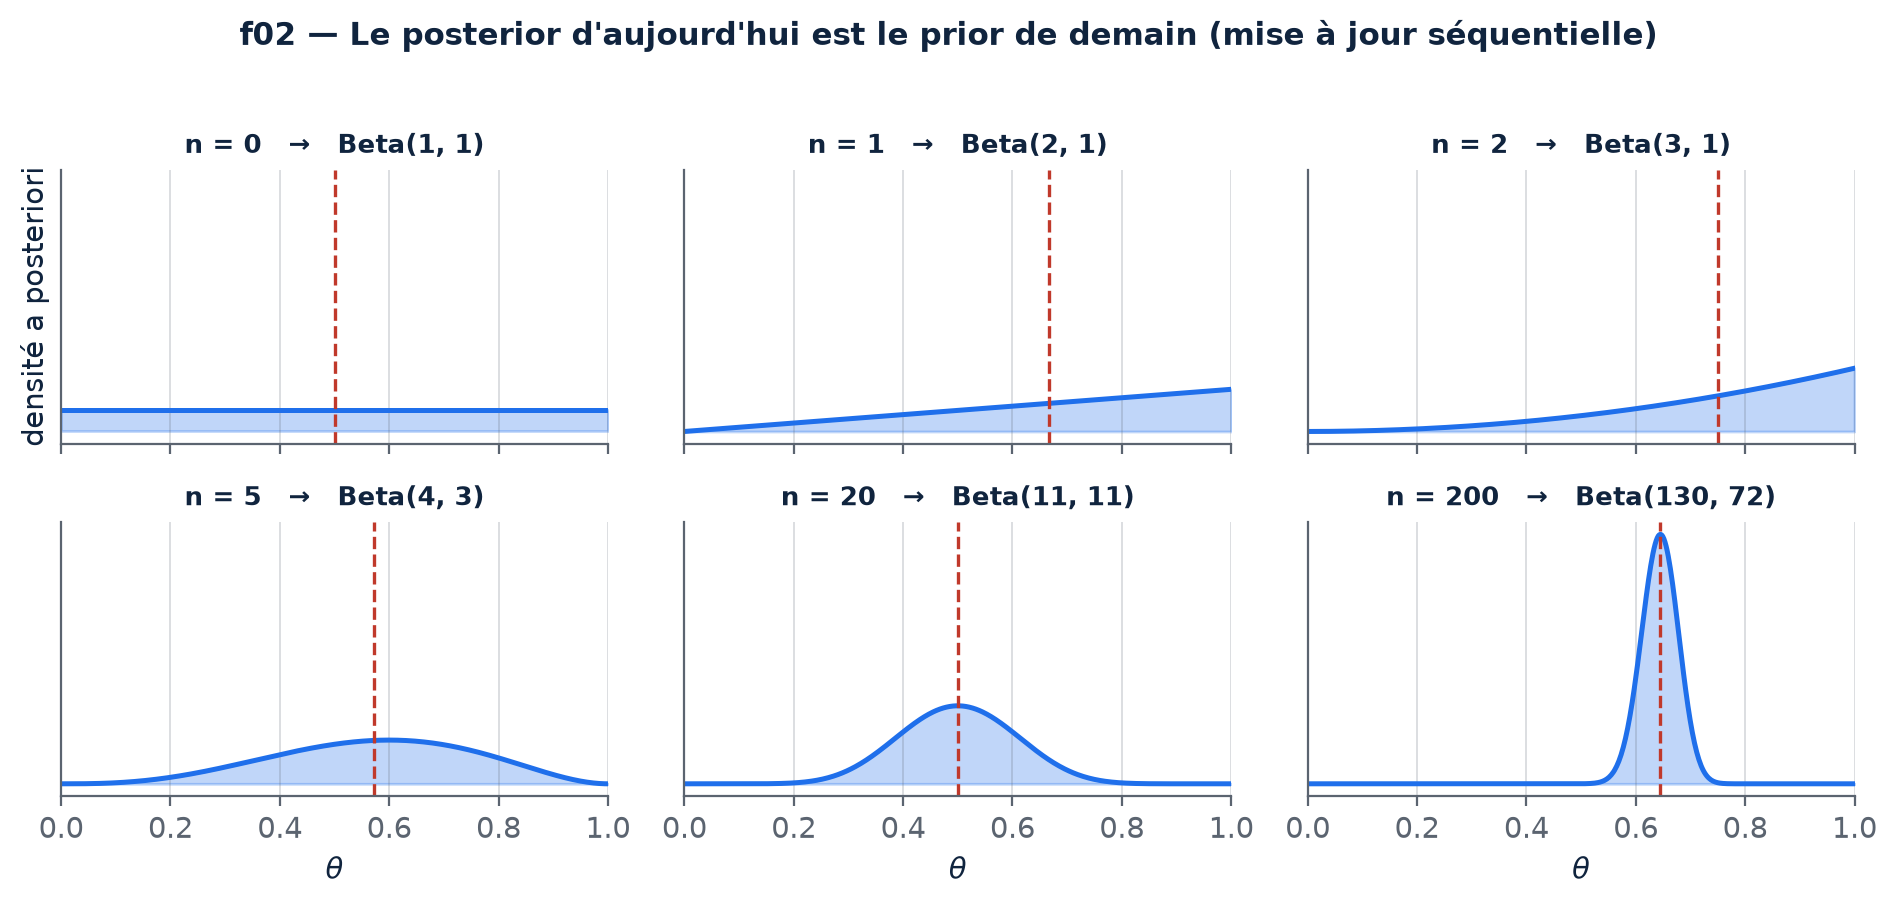
\includegraphics[width=.82\textwidth]{f02_beta_updating.png}
\end{center}
\vspace{-1mm}
\centering\footnotesize
Simulation réelle : 200 lancers d'une pièce biaisée ($p = 0{,}65$), prior Beta$(1,1)$.
La dispersion se resserre comme $1/\sqrt{n}$ : c'est la \emph{vitesse d'apprentissage}.
\end{frame}
